\chapter{Smooth Functions}
\label{ch: smooth_func}

\graphicspath{{Figures/Smooth_func/}{./}} 
\textbf{This is a section not a chapter}

\section{Smooth Functions}
The pinball loss function we use for the SGD quantile estimation is convex but not smooth. 
Theoretically, however, both SGD and SAG methods need smoothness for the guarantee of convergence. Although the practical experiments have shown that there is evidence of convergence in final performance, it remains a serious problem for our SGD quantile estimation methods. In this section, we present the analysis on the non-smoothness problem, followed by the potential solutions and further discussions on them.

\subsection{The Pinball Loss Functions}
The pinball loss function evaluates the loss from a data point $x$ for estimation of the $\tau$-quantile.

\textbf{quote the equation of pinball loss function and it's derivative}

The fact that the pinball loss function is not differentiable at $x= 0$ has became a problem for the stochastic gradient descent which uses derivatives of object functions.

\begin{figure*}[h!]
	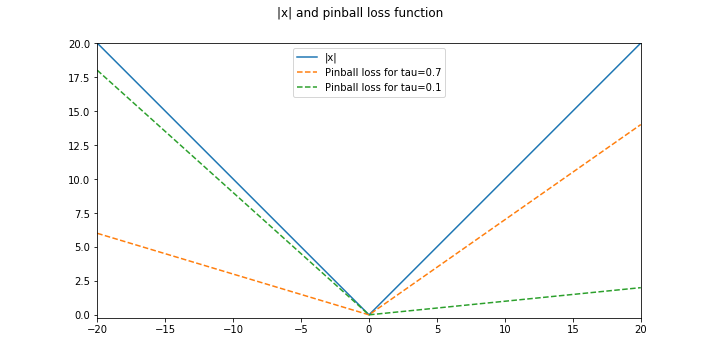
\includegraphics[width=1\columnwidth]{abs_pinball.png}
	\caption{Comparison between $|x|$ and the pinball loss function with different $\tau$ values}
\end{figure*}

The absolute function and the pinball loss function are obviously very much alike. In fact, with simple manipulation, the pinball loss function can be written in the form of absolute function as 
\begin{equation}
    l_\tau(x) = 
    \begin{cases}
        \tau \cdot |x| & {x \geq 0} \\
        (1-\tau) \cdot |x| & \text{otherwise}
    \end{cases}
\end{equation}
The pinball loss function is the combination of $|x|$ on the two parts $x<0$ and $x>0$ with different constant scale. 
If the derivative of the smooth function for $|x|$ at $x=0$ is $0$, we can also use the same approximation function respectively for the two parts of the pinball loss.
\\\\
In section \ref{subsec: smooth_sqrt} and \ref{subsec: smooth_new}, we show two approximation functions with regards to the absolute function $f = |x|$, along with the application of the approximations on the pinball loss function.

\subsection{Smooth function 1: a simple approximation}
\label{subsec: smooth_sqrt}

For $f = |x|$, a common and simple smooth approximation is $
    f = \sqrt{x^2 + \mu^2}
$.
 The convergence towards the absolute function is then proved by \citeauthor{voroninConvolutionBasedSmooth2015a}\cite{voroninConvolutionBasedSmooth2015a} that 
\begin{equation}
    ||x| - \sqrt{x^2 + \mu^2}| \leq \mu \text{  where } \mu > 0 \in \mathbb{R}
\end{equation}
\\
The smooth function application on the pinball loss function is:
\begin{equation}
    l_\tau(x) \approx 
    \begin{cases}
        \tau \cdot \sqrt{x^2 + \mu^2} & {x \geq 0} \\
        (1-\tau) \cdot \sqrt{x^2 + \mu^2} & {x < 0}
    \end{cases}
\end{equation}
and the derivative is
\begin{equation}
    l_\tau\prime(x) \approx 
    \begin{cases}
        \tau \cdot \frac{x}{\sqrt{x^2 + \mu^2}} & {x > 0} \\
        0 & {x=0} \\
        (1-\tau) \cdot \frac{x}{\sqrt{x^2 + \mu^2}} & {x<0}
    \end{cases}
\end{equation}
\subsection{Smooth function 2: a transcendental approximation}
\label{subsec: smooth_new}

For a better approximation accuracy, \citeauthor{bagulSMOOTHTRANSCENDENTALAPPROXIMATION2017}\cite{bagulSMOOTHTRANSCENDENTALAPPROXIMATION2017} proposes a new transcendental approximation function 
 \begin{equation}
    g(x) = x \cdot \tanh(x/\mu) \text{  where } \mu > 0 \in \mathbb{R}
 \end{equation}
which also satisfies
\begin{equation}
    ||x| - x \cdot tanh(\frac{x}{\mu})| < \mu
\end{equation}
The derivative of the approximation is
\begin{equation}
    \frac{dg(x)}{dx} = \frac{x}{\mu} \cdot sech^2 (\frac{x}{\mu}) + tanh(\frac{x}{\mu})
\end{equation}
For the pinball loss function, we now have its smooth function in the form:
\begin{equation}
    l_\tau(x) \approx 
    \begin{cases}
        \tau \cdot x \cdot \tanh(x/\mu) & {x\geq 0}\\
        (1-\tau) \cdot x \cdot \tanh(x/\mu) & {x < 0}
    \end{cases}
\end{equation}
and the derivative is
\begin{equation}
\label{eq:smooth_new_d}
    l_\tau\prime(x) \approx 
    \begin{cases}
        \tau \cdot \frac{x}{\mu} \cdot sech^2 (\frac{x}{\mu}) + tanh(\frac{x}{\mu}) & {x\geq 0}\\
        0 & {x=0}\\
        (1-\tau) \cdot \frac{x}{\mu} \cdot sech^2 (\frac{x}{\mu}) + tanh(\frac{x}{\mu}) & {x < 0}
    \end{cases}
\end{equation}
\subsection{Discussion and Conclusion}

In this part, we will compare the two alternative smooth functions in the following aspects: computer efficiency, approximation accuracy and
convexity. 
\begin{itemize}
    \item Computation efficiency: \\
    It is proved by \citeauthor{ramirezX2MostComputationally2014}\cite{ramirezX2MostComputationally2014} that $f = \sqrt{x^2 + \mu^2}$ is the most computationally efficient smooth approximation to $|x|$.
    
    On the other hand, we can see from equation \ref{eq:smooth_new_d}, the derivative for $g(x) = x · \tanh(x/\mu)$ is more difficult to compute.
    \item Approximation accuracy: \\
    The following plots show intuitively how fast the two smooth functions approach to $|x|$ for $\mu = 0.01$ and $\mu = 0.001$.
    
    \begin{figure*}[h!]
        \includegraphics[width=1\columnwidth]{{mu_0.001}.png}
        \caption{Comparison between the two smooth functions when $\mu = 0.001$}
    \end{figure*}

    \begin{figure*}[h!]
        \includegraphics[width=1\columnwidth]{{mu_0.0001}.png}
        \caption{Comparison between the two smooth functions when $\mu = 0.0001$}
    \end{figure*}

    We can see $ x \cdot \tanh(x/\mu)$ has a better accuracy.

    \item Convexity\\
    $f = \sqrt{x^2 + \mu^2}$ is convex and  $g(x) = x · \tanh(x/\mu)$ is not.
\end{itemize}

\textbf{Here we need a conclusion}
\textbf{Picure position is not forced to go with text position :(}


